\documentclass[tikz,border=10pt]{standalone}
% Scale s = 0.012882 (STYLE METRICS), centred on ink bbox centre
\begin{document}
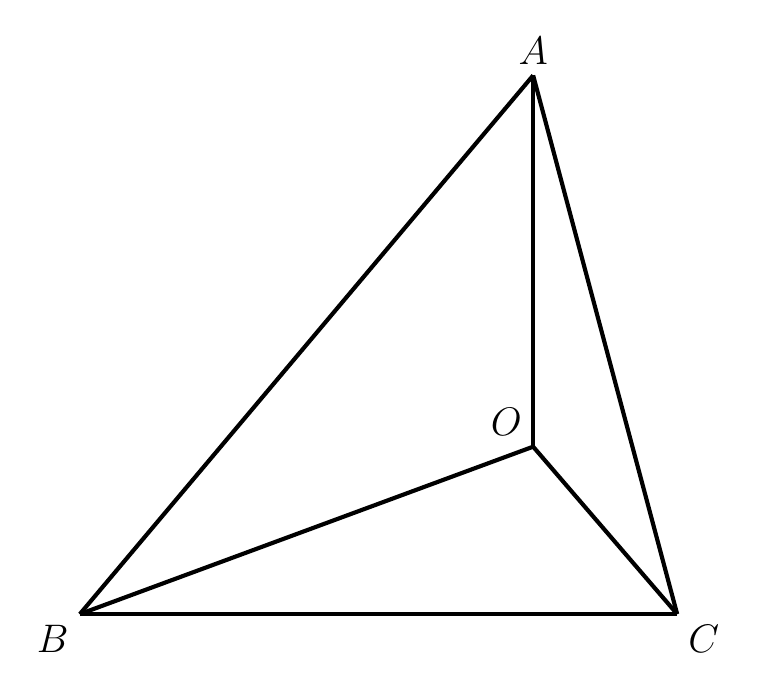
\begin{tikzpicture}[line join=round, line width=1.5pt]
  % Named coordinates (converted from pixels)
  \coordinate (A) at (1.964, 3.427);
  \coordinate (B) at (-3.793, -3.414);
  \coordinate (C) at (3.793, -3.414);
  \coordinate (O) at (1.964, -1.288);

  % Triangle sides
  \draw (A) -- (B);
  \draw (B) -- (C);
  \draw (C) -- (A);

  % Segments from interior point O
  \draw (O) -- (A);
  \draw (O) -- (B);
  \draw (O) -- (C);

  % Labels
  \node[above, font=\fontsize{15}{18}\selectfont] at (A) {$A$};
  \node[below left, font=\fontsize{15}{18}\selectfont] at (B) {$B$};
  \node[below right, font=\fontsize{15}{18}\selectfont] at (C) {$C$};
  \node[above left, font=\fontsize{15}{18}\selectfont] at (O) {$O$};
\end{tikzpicture}
\end{document}